\clearpage

\subsection{Translucent with 1+1 Protection}\label{ILP_Transluc_Protection}
\begin{tcolorbox}	
\begin{tabular}{p{2.75cm} p{0.2cm} p{10.5cm}} 	
\textbf{Student Name}  &:& Tiago Esteves    (October 03, 2017 - )\\
\textbf{Goal}          &:& Implement the ILP model for the translucent transport mode with 1 plus 1 protection.
\end{tabular}
\end{tcolorbox}

\subsubsection{Model description}

Here, in this case, we must take into account table \ref{description_transluc}, previously mentioned, in order to better understand the objective function.\\

Before carrying out the description of the objective function we must take into account the following particularity of this mode of transport:
\begin{itemize}
  \item $N_{OXC,n}$ = 1, \quad $\forall$ n that process traffic
  \item $N_{EXC,n}$ = 1, \quad $\forall$ n that process traffic
\end{itemize}

\vspace{11pt}
The objective function of following the ILP is a minimization of the CAPEX through the equation \ref{Capex} where in this case for the cost of nodes we have in consideration electric \ref{Capex_Node_EXC} and optical cost \ref{Capex_Node_OXC}. In this case the value of $P_{exc,c,n}$ is obtained by equation \ref{EXC_pexc1_translucp} for short-reach and by the equation \ref{EXC_pexc2_translucp} for long-reach and the value of $P_{oxc,n}$ is obtained by equation \ref{OXC_poxc_translucp}.\\

The equation \ref{EXC_pexc1_translucp} refers to the number of sort-reach ports of the electrical switch with bit-rate $c$ in node $n$, $P_{exc,c,n}$, i.e. the number of tributary ports with bit-rate $c$ in node $n$ which can be calculated as

\begin{equation}
P_{exc,c,n} = \sum_{d=1}^{N} D_{nd,c}
\label{EXC_pexc1_translucp}
\end{equation}

\vspace{11pt}
\noindent
where $D_{nd,c}$ are the client demands between nodes $n$ and $d$ with bit rate $c$.\\

In this case there is the following particularity:
\begin{itemize}
  \item When $n$=$d$ the value of client demands is always zero, i.e, $D_{nn,c}=0$
\end{itemize}

\vspace{11pt}
As previously mentioned, the equation \ref{EXC_pexc2_translucp} refers to the number of long-reach ports of the electrical switch with bit-rate -1 in node n, $P_{exc,-1,n}$, i.e. the number of add ports of node n which can be calculated as

\begin{equation}
P_{exc,-1,n} = \sum_{k=1}^{N} \lambda_{nk}
\label{EXC_pexc2_translucp}
\end{equation}

\vspace{11pt}
\noindent
where $\lambda_{nk}$ is the number of optical channels between lightpath $n$ and node $k$.\\

The equation \ref{OXC_poxc_translucp} refers to the number of ports in optical switch in node n, $P_{oxc,n}$, i.e. the number of line ports and the number of adding ports of node n which can be calculated as

\begin{equation}
P_{oxc,n} = \sum_{j=1}^{N} f_{nj}^{pk} + \sum_{k=1}^{N} \lambda_{nk}
\label{OXC_poxc_translucp}
\end{equation}

\vspace{11pt}
\noindent
where $f_{nj}^{pk}$ refers to the number of line ports for all lightpath pairs $(p,k)$ and $\lambda_{nk}$ refers to the number of add ports.\\

The objective function, to be minimized, is the expression \ref{ILPOpaque_CAPEX}, i.e.,
\begin{equation*}
  minimize \qquad \Big\{ \quad C_C \quad \Big\}
\end{equation*}

$subject$ $to$
\begin{equation}
\sum_{k\textbackslash \{o\}} Ls_{pk}^{odc} = D_{odc} \qquad \qquad \qquad \qquad \qquad \qquad \qquad
\forall(o,d,c) : o < d, \forall p: p = o
\label{ILPTranslucp1}
\end{equation}
\noindent
This are the virtual flow conservation constraints and ensure that, for each $(o,d)$ pair, we route client demand units of flow from node $o$ to node $d$, the source node sends client demand units of flow.

\begin{equation}
\sum_{k\textbackslash \{p,o\}} Ls_{pk}^{odc} = \sum_{k\textbackslash \{p,d\}} Ls_{kp}^{odc} \qquad \qquad \qquad \qquad
\forall(o,d,c) : o < d, \forall p: p \neq o,d
\label{ILPTranslucp2}
\end{equation}
\noindent
This constraint ensure that the remaining nodes, being neither origin or destination, the receive flow have to be send.

\begin{equation}
\sum_{k\textbackslash \{d\}} Ls_{kp}^{odc} = D_{odc} \qquad \qquad \qquad \qquad \qquad \qquad \qquad \qquad
\forall(o,d,c) : o < d, \forall p: p = d
\label{ILPTranslucp3}
\end{equation}
\noindent
This are the virtual flow conservation constraints and ensure that, for each $(o,d)$ pair, we route client demand units of flow from node $o$ to node $d$, the destination node has to receive those client demand units of flow.

\begin{equation}
\sum_{k\textbackslash \{o\}} Lsp_{pk}^{odc} = D_{odc} \qquad \qquad \qquad \qquad \qquad \qquad \qquad
\forall(o,d,c) : o < d, \forall p: p = o
\label{ILPTranslucp1p}
\end{equation}
\noindent
This are the virtual protection flow conservation constraints and ensure that, for each $(o,d)$ pair, we route client demand units of flow from node $o$ to node $d$, the source node sends client demand units of flow.

\begin{equation}
\sum_{k\textbackslash \{p,o\}} Lsp_{pk}^{odc} = \sum_{k\textbackslash \{p,d\}} Lsp_{kp}^{odc} \qquad \qquad \qquad \qquad
\forall(o,d,c) : o < d, \forall p: p \neq o,d
\label{ILPTranslucp2p}
\end{equation}
\noindent
This constraint ensure that the remaining nodes for protection, being neither origin or destination, the receive flow have to be send.

\begin{equation}
\sum_{k\textbackslash \{d\}} Lsp_{kp}^{odc} = D_{odc} \qquad \qquad \qquad \qquad \qquad \qquad \qquad \qquad
\forall(o,d,c) : o < d, \forall p: p = d
\label{ILPTranslucp3p}
\end{equation}
\noindent
This are the virtual protection flow conservation constraints and ensure that, for each $(o,d)$ pair, we route client demand units of flow from node $o$ to node $d$, the destination node has to receive those client demand units of flow.

\begin{equation}
(Ls_{pk}^{odc} + Lsp_{pk}^{odc}) \leq D_{odc} \qquad \qquad \qquad \qquad \qquad \qquad \qquad \qquad
\forall (p,k), \forall(o,d,c) : o < d
\label{ILPTranslucpX}
\end{equation}
\noindent
This constraint assures us that the variable $Ls_{pk}^{odc}$ (working flow) and $Lsp_{pk}^{odc}$ (protection flow) are different.

\begin{equation}
\sum_{o=1} \sum_{d=o+1} \sum_{c=1} B(c)(Ls_{pk}^{odc} + Ls_{kp}^{odc} + Lsp_{pk}^{odc} + Lsp_{kp}^{odc}) \leq  \tau \lambda_{pk} \qquad \qquad
\forall (p,k) : p < k
\label{ILPTranslucp4}
\end{equation}
\noindent
This restriction is considered grooming constraint and the variable $\tau$ is always 100 Gbits/s.

\begin{equation}
\sum_{j\textbackslash \{p\}} f_{ij}^{pk} = \lambda_{pk}  \qquad \qquad \qquad \qquad \qquad \qquad \qquad \qquad \qquad
\forall(p,k) : p < k, \forall i: i = p
\label{ILPTranslucp6}
\end{equation}
\noindent
This constraint are equal to the constraint \ref{ILPOpaque1_CAPEX} assuming that Z variable has the value of number of optical channels between this demand for all bidirectional links.

\begin{equation}
\sum_{j\textbackslash \{p\}} f_{ij}^{pk} = \sum_{j\textbackslash \{k\}} f_{ji}^{pk} \qquad \qquad \qquad \qquad \qquad \qquad \qquad \qquad
\forall(p,k) : p < k, \forall i: i \neq p,k
\label{ILPTranslucp7}
\end{equation}
\noindent
This constraint are equal to the constraint \ref{ILPOpaque2_CAPEX}.

\begin{equation}
\sum_{j\textbackslash \{k\}} f_{ji}^{pk} = \lambda_{pk}  \qquad \qquad \qquad \qquad \qquad \qquad \qquad \qquad \qquad
\forall(p,k) : p < k, \forall i: i = k
\label{ILPTranslucp8}
\end{equation}
\noindent
This constraint are equal to the constraint \ref{ILPOpaque3_CAPEX} assuming that Z variable has the value of number of optical channels between this demand for all bidirectional links.
\newpage
\begin{equation}
\sum_{p=1} \sum_{k=p+1} \left( f_{ij}^{pk} + f_{ji}^{pk}\right) \leq K_{ij} G_{ij} L_{ij} \qquad \qquad \qquad \qquad \qquad \qquad \qquad
\forall (i,j) : i < j
\label{ILPTranslucp9}
\end{equation}
\noindent
This restriction answers capacity constraint problem. Then, total flows must be less or equal to the capacity of network links. For any situation the maximum number of optical channels supported by each transmission system is 100, i.e., $K_{ij}$ = 100.

\begin{equation}
f_{ij}^{pk} , f_{ji}^{pk} , Ls_{pk}^{odc} , Ls_{kp}^{odc} , \lambda_{pk} \in \mathbb{N}   \qquad \qquad \qquad \qquad \qquad
\forall(i,j) : i < j, \forall(o,d) : o < d
\label{ILPTranslucp10}
\end{equation}
\noindent
This constraint defines that these variables must be a counting number.

\begin{equation}
L_{i,j} \in \{0,1\} \qquad \qquad \qquad \qquad \qquad \qquad \qquad \qquad \qquad \qquad \qquad \qquad \qquad \qquad
\forall(i,j)
\label{ILPTransluc11}
\end{equation}
\noindent
Last constraint refers to the use of the link where this variable can be zero if it is not being used or one if is being used.

\vspace{18pt}
\subsubsection{Result description}

To perform the calculations using the implementation of the models described previously it is necessary to use a mathematical software tool. For this we will use MATLAB which is ideal for dealing with linear programming problems and can call the LPsolve through an external interface.
We already have all the necessary to obtain the CAPEX value for the reference network \ref{Reference_Network_Topology}. As described in the subsection of network traffic \ref{Reference_Network_Traffic}, we have three values of network traffic so we have to obtain three different CAPEX. The value of the CAPEX of the network will be calculated based on the costs of the equipment present in the table \ref{table_cost_ilp}.\\

\textbf{Low Traffic Scenario:}\\

In this scenario we have to take into account the traffic calculated in \ref{low_scenario}. In a first phase we will show the various existing topologies of the network. The first are the allowed topologies, physical and optical topology, the second are the logical topology for all ODUs and finally the resulting physical and optical topology.\\

\newpage
\begin{figure}[h!]
\centering
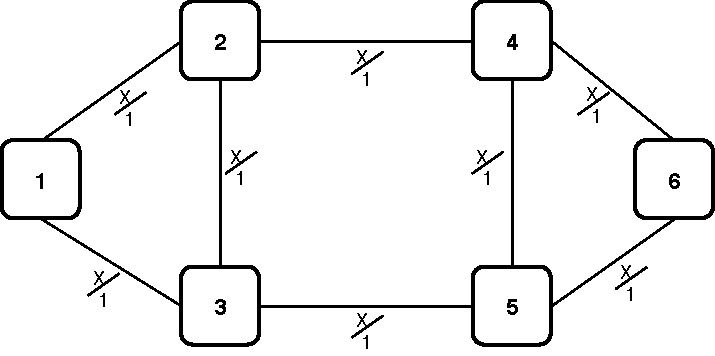
\includegraphics[width=13cm]{sdf/ilp/translucent_protection/figures/allowed_physical_topology}
\caption{Allowed physical topology. The allowed physical topology is defined by the duct and sites in the field. It is assumed that each duct supports up to 1 bidirectional transmission system and each site supports up to 1 node.}
\label{allowed3_physical_protectionlow}
\end{figure}

\vspace{20pt}
\begin{figure}[h!]
\centering
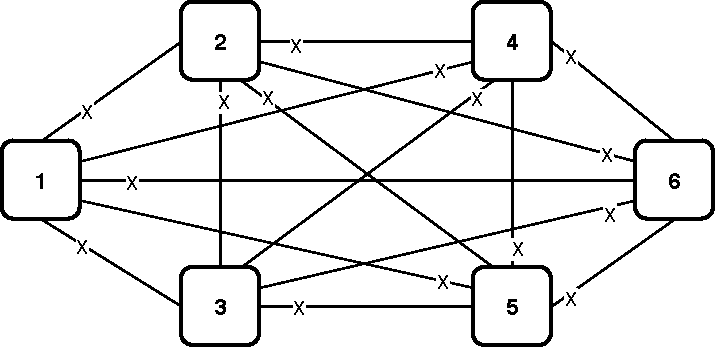
\includegraphics[width=13cm]{sdf/ilp/translucent_protection/figures/allowed_optical_topology}
\caption{Allowed optical topology. The allowed optical topology is defined by the transport mode (translucent transport mode in this case). It is assumed that each connections between demands supports up to 100 lightpaths.}
\label{allowed3_optical_protectionlow}
\end{figure}

\newpage
\begin{figure}[h!]
\centering
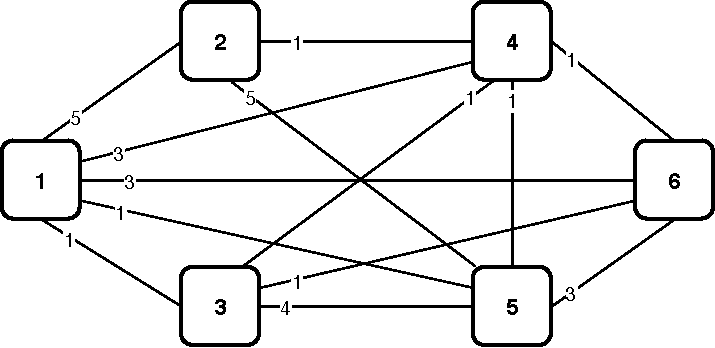
\includegraphics[width=12cm]{sdf/ilp/translucent_protection/figures/logical_topology_ODU0_low}
\caption{ODU0 logical topology defined by the ODU0 traffic matrix.}
\label{logical3_ODU0_protectionlow}
\end{figure}

\begin{figure}[h!]
\centering
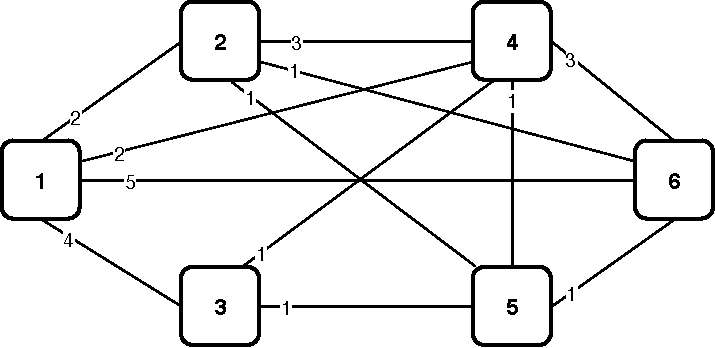
\includegraphics[width=12cm]{sdf/ilp/translucent_protection/figures/logical_topology_ODU1_low}
\caption{ODU1 logical topology defined by the ODU1 traffic matrix.}
\label{logical3_ODU1_protectionlow}
\end{figure}

\begin{figure}[h!]
\centering
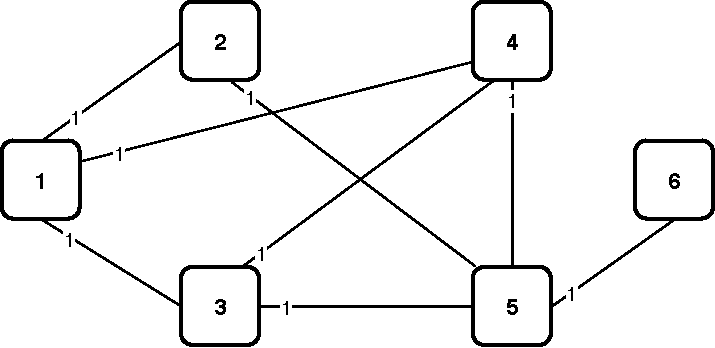
\includegraphics[width=12cm]{sdf/ilp/translucent_protection/figures/logical_topology_ODU2_low}
\caption{ODU2 logical topology defined by the ODU2 traffic matrix.}
\label{logical3_ODU2_protectionlow}
\end{figure}

\begin{figure}[h!]
\centering
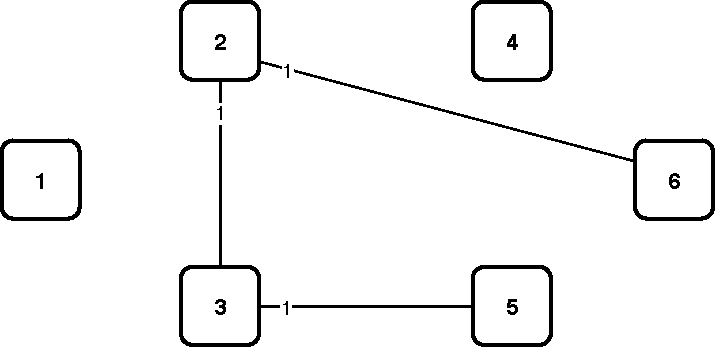
\includegraphics[width=12cm]{sdf/ilp/translucent_protection/figures/logical_topology_ODU3_low}
\caption{ODU3 logical topology defined by the ODU3 traffic matrix.}
\label{logical3_ODU3_protectionlow}
\end{figure}

\begin{figure}[h!]
\centering
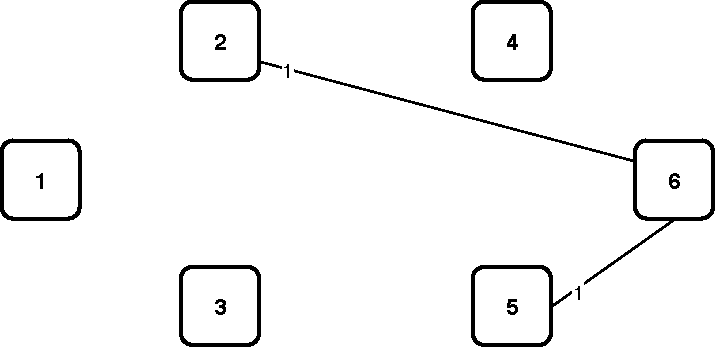
\includegraphics[width=12cm]{sdf/ilp/translucent_protection/figures/logical_topology_ODU4_low}
\caption{ODU4 logical topology defined by the ODU4 traffic matrix.}
\label{logical3_ODU4_protectionlow}
\end{figure}

\begin{figure}[h!]
\centering
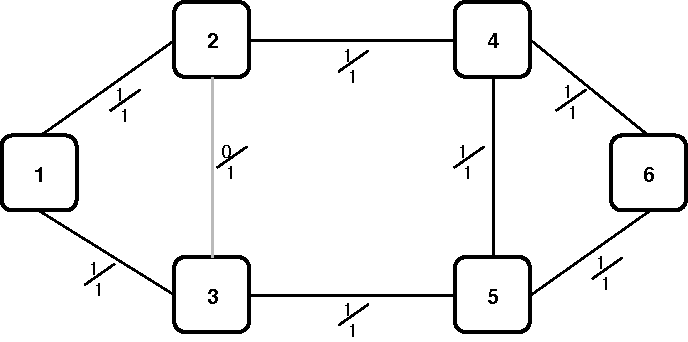
\includegraphics[width=12cm]{sdf/ilp/translucent_protection/figures/physical_topology_low}
\caption{Physical topology after dimensioning.}
\label{physical3_protectionlow}
\end{figure}
\newpage
\begin{figure}[h!]
\centering
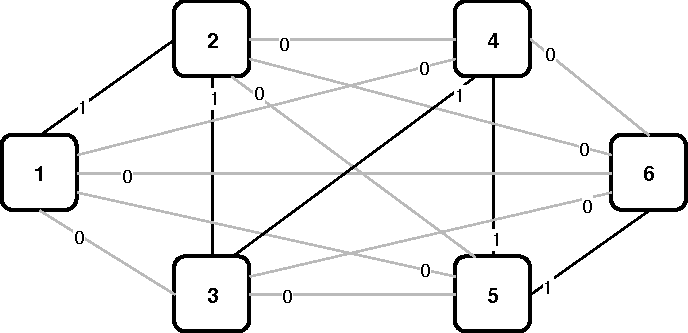
\includegraphics[width=12cm]{sdf/ilp/translucent_protection/figures/optical_topology_low}
\caption{Optical topology after dimensioning.}
\label{optical3_protectionlow}
\end{figure}

\vspace{15pt}
In table \ref{link_transluc_protec_ref_low} we can see the number of optical channels calculated using \ref{Capex_Link} and \ref{ILPOpaque_CAPEX} and the number of amplifiers for each link calculated using \ref{Capex_amplifiers}. In the case where there are no optical channels we assume that the number of amplifiers is zero.\\

\begin{table}[h!]
\centering
\begin{tabular}{|| c | c | c ||}
 \hline
 \multicolumn{3}{|| c ||}{Information regarding links} \\
 \hline
 \hline
 Bidirectional Link & Optical Channels & Amplifiers\\
 \hline
 Node 1 <-> Node 2 & 1 & 4 \\
 Node 1 <-> Node 3 & 1 & 6 \\
 Node 2 <-> Node 3 & 0 & 0 \\
 Node 2 <-> Node 4 & 1 & 6 \\
 Node 3 <-> Node 5 & 2 & 8 \\
 Node 4 <-> Node 5 & 1 & 1 \\
 Node 4 <-> Node 6 & 2 & 7 \\
 Node 5 <-> Node 6 & 2 & 3 \\
 \hline
\end{tabular}
\caption{Table with information regarding links for translucent mode with 1+1 protection.}
\label{link_transluc_protec_ref_low}
\end{table}

\vspace{15pt}
In table \ref{node_transluc_protec_ref_low} we can see the resulting nodal degree at the physical layer, calculated based on the number of connections that the node in question performs, the number of line ports and add ports using \ref{OXC_poxc_transluc} the number of long-reach transponders using \ref{EXC_pexc2_transluc} and the number of tributary ports using \ref{EXC_pexc1_transluc}.\\
\newpage
\begin{table}[h!]
\centering
\begin{tabular}{|| c | c | c | c | c | c ||}
 \hline
 \multicolumn{6}{|| c ||}{Information regarding nodes} \\
 \hline
 \hline
 \multicolumn{2}{|| c |}{ } & \multicolumn{2}{ c |}{Electrical part} & \multicolumn{2}{ c ||}{Optical part} \\
 \hline
 Node & Resulting Nodal Degree & Tributary Ports & LR Transponders & Add Ports & Line Ports\\
 \hline
 1 & 2 & 29 & 2 & 2 & 2 \\
 2 & 2 & 23 & 2 & 2 & 2 \\
 3 & 2 & 18 & 3 & 3 & 3 \\
 4 & 3 & 20 & 4 & 4 & 4 \\
 5 & 3 & 24 & 3 & 3 & 5 \\
 6 & 2 & 22 & 4 & 4 & 4 \\
\hline
\end{tabular}
\caption{Table with information regarding nodes for translucent mode with 1+1 protection.}
\label{node_transluc_protec_ref_low}
\end{table}

Through the information obtained previously on the nodes we can now create tables with detailed information about each node. In each table mentioned below we can see how many ports are connected to a given node and its bit rate (in relation to the line ports) and how many ports are assigned to each different bit rate (in relation to the tributary ports).\\

\begin{table}[h!]
\centering
\begin{tabular}{|| c | c | c ||}
 \hline
 \multicolumn{3}{|| c ||}{Detailed description of Node 1} \\
 \hline
 \hline
 Electrical part & Number of total demands & Bit rate \\
 \hline
\multirow{3}{*}{29 tributary ports} & 13 & ODU0 \\
 & 13 & ODU1 \\
 & 3 & ODU2 \\
 \hline
  & Node<--Optical Channels-->Node & Bit rate \\
 \hline
 \multirow{2}{*}{2 LR Transponders} & 1  <---- 1 ---->  2 & \multirow{2}{*}{100 Gbits/s} \\
  & 1  <---- 1 ---->  3 & \\
 \hline
 \hline
 Optical part & Node<--Optical Channels-->Node & Bit rate \\
 \hline
 \multirow{2}{*}{2 add ports} & 1  <---- 1 ---->  2 & \multirow{4}{*}{100 Gbits/s} \\
  & 1  <---- 1 ----> 3 & \\ \cline{1-2}
 \multirow{2}{*}{2 line ports} & 1  <---- 1 ---->  2 & \\
  & 1  <---- 1 ----> 3 & \\
\hline
\end{tabular}
\caption{Table with detailed description of node 1. The number of demands is distributed to the various destination nodes, this distribution can be observed in section \ref{low_scenario}.}
\end{table}
\newpage
\begin{table}[h!]
\centering
\begin{tabular}{|| c | c | c ||}
 \hline
 \multicolumn{3}{|| c ||}{Detailed description of Node 2} \\
 \hline
 \hline
 Electrical part & Number of total demands & Bit rate \\ \hline
\multirow{5}{*}{23 tributary ports} & 11 & ODU0 \\
 & 7 & ODU1 \\
 & 2 & ODU2 \\
 & 2 & ODU3 \\
 & 1 & ODU4 \\
 \hline
  & Node<--Optical Channels-->Node & Bit rate \\
  \hline
\multirow{2}{*}{2 LR Transponders} & 2  <---- 1 ---->  1 & \multirow{2}{*}{100 Gbits/s} \\
  & 2  <---- 1 ---->  4 & \\
 \hline
 \hline
 Optical part & Node<--Optical Channels-->Node & Bit rate \\
 \hline
 \multirow{2}{*}{2 add ports} & 2  <---- 1 ---->  1 & \multirow{4}{*}{100 Gbits/s} \\
  & 2  <---- 1 ---->  4 & \\ \cline{1-2}
 \multirow{2}{*}{2 line ports} & 2  <---- 1 ---->  1 & \\
  & 2  <---- 1 ---->  4 & \\
\hline
\end{tabular}
\caption{Table with detailed description of node 2. The number of demands is distributed to the various destination nodes, this distribution can be observed in section \ref{low_scenario}.}
\end{table}
\newpage
\begin{table}[h!]
\centering
\begin{tabular}{|| c | c | c ||}
 \hline
 \multicolumn{3}{|| c ||}{Detailed description of Node 3} \\
 \hline
 \hline
 Electrical part & Number of total demands & Bit rate \\
 \hline
 \multirow{4}{*}{18 tributary ports} & 7 & ODU0 \\
 & 6 & ODU1\\
 & 3 & ODU2\\
 & 2 & ODU3\\
 \hline
  & Node<--Optical Channels-->Node & Bit rate \\ \hline
 \multirow{3}{*}{3 LR Transponders} & 3  <---- 1 ---->  1 & \multirow{3}{*}{100 Gbits/s} \\
  & 3  <---- 1 ---->  5 & \\
  & 3  <---- 1 ---->  6 & \\
 \hline
 \hline
 Optical part & Node<--Optical Channels-->Node & Bit rate \\
 \hline
 \multirow{3}{*}{3 add ports} & 3  <---- 1 ---->  1 & \multirow{6}{*}{100 Gbits/s} \\
  & 3  <---- 1 ---->  5 & \\
  & 3  <---- 1 ---->  6 & \\  \cline{1-2}
 \multirow{3}{*}{3 line ports} & 3  <---- 1 ---->  1 & \\
  & 3  <---- 1 ---->  5 & \\
  & 3  <---- 1 ---->  6 & \\
\hline
\end{tabular}
\caption{Table with detailed description of node 3. The number of demands is distributed to the various destination nodes, this distribution can be observed in section \ref{low_scenario}.}
\end{table}
\newpage
\begin{table}[h!]
\centering
\begin{tabular}{|| c | c | c ||}
 \hline
 \multicolumn{3}{|| c ||}{Detailed description of Node 4} \\
 \hline
 \hline
 Electrical part & Number of total demands & Bit rate \\ \hline
\multirow{3}{*}{20 tributary ports} & 7 & ODU0 \\
 & 10 & ODU1 \\
 & 3 & ODU2 \\
 \hline
  & Node<--Optical Channels-->Node & Bit rate \\ \hline
 \multirow{3}{*}{4 LR Transponders} & 4  <---- 1 ---->  2 & \multirow{3}{*}{100 Gbits/s} \\
  & 4  <---- 1 ---->  5 & \\
  & 4  <---- 2 ---->  6 & \\
 \hline
 \hline
 Optical part & Node<--Optical Channels-->Node & Bit rate \\
 \hline
 \multirow{3}{*}{4 add ports} & 4  <---- 1 ---->  2 & \multirow{6}{*}{100 Gbits/s} \\
  & 4  <---- 1 ---->  5 & \\
  & 4  <---- 2 ---->  6 & \\ \cline{1-2}
 \multirow{3}{*}{4 line ports} & 4  <---- 1 ---->  2 & \\
  & 4  <---- 1 ---->  5 & \\
  & 4  <---- 2 ---->  6 & \\
\hline
\end{tabular}
\caption{Table with detailed description of node 4. The number of demands is distributed to the various destination nodes, this distribution can be observed in section \ref{low_scenario}.}
\end{table}
\newpage
\begin{table}[h!]
\centering
\begin{tabular}{|| c | c | c ||}
 \hline
 \multicolumn{3}{|| c ||}{Detailed description of Node 5} \\
 \hline
 \hline
 Electrical part & Number of total demands & Bit rate \\ \hline
\multirow{5}{*}{24 tributary ports} & 14 & ODU0 \\
 & 4 & ODU1 \\
 & 4 & ODU2 \\
 & 1 & ODU3 \\
 & 1 & ODU4 \\
 \hline
  & Node<--Optical Channels-->Node & Bit rate \\ \hline
 \multirow{3}{*}{3 LR Transponders} & 5  <---- 1 ---->  3 & \multirow{3}{*}{100 Gbits/s} \\
  & 5  <---- 1 ---->  4 & \\
  & 5  <---- 1 ---->  6 & \\
 \hline
 \hline
 Optical part & Node<--Optical Channels-->Node & Bit rate \\
 \hline
 \multirow{3}{*}{3 add ports} & 5  <---- 1 ---->  3 & \multirow{7}{*}{100 Gbits/s} \\
  & 5  <---- 1 ---->  4 & \\
  & 5  <---- 1 ---->  6 & \\ \cline{1-2}
 \multirow{4}{*}{5 line ports} & 5  <---- 1 ---->  3 & \\
  & 5  <---- 1 ---->  4 & \\
  & 5  <---- 1 ---->  6 & \\
  & 3  <---- 1 ---->  6 & \\
  \hline
\end{tabular}
\caption{Table with detailed description of node 5. The number of demands is distributed to the various destination nodes, this distribution can be observed in section \ref{low_scenario}.}
\end{table}
\newpage
\begin{table}[h!]
\centering
\begin{tabular}{|| c | c | c ||}
 \hline
 \multicolumn{3}{|| c ||}{Detailed description of Node 6} \\
 \hline
 \hline
 Electrical part & Number of total demands & Bit rate \\ \hline
\multirow{5}{*}{22 tributary ports} & 8 & ODU0 \\
 & 10 & ODU1 \\
 & 1 & ODU2 \\
 & 1 & ODU3 \\
 & 2 & ODU4 \\
 \hline
  & Node<--Optical Channels-->Node & Bit rate \\ \hline
 \multirow{3}{*}{4 LR Transponders} & 6  <---- 1 ---->  3 & \multirow{3}{*}{100 Gbits/s} \\
  & 6  <---- 2 ---->  4 & \\
  & 6  <---- 1 ---->  5 & \\
 \hline
 Optical part & Node<--Optical Channels-->Node & Bit rate \\
 \hline
 \multirow{3}{*}{4 add ports} & 6  <---- 1 ---->  3 & \multirow{3}{*}{100 Gbits/s} \\
  & 6  <---- 2 ---->  4 & \\
  & 6  <---- 1 ---->  5 & \\ \cline{1-2}
 \multirow{3}{*}{4 line ports} & 6  <---- 1 ---->  3 & \\
  & 6  <---- 2 ---->  4 & \\
  & 6  <---- 1 ---->  5 & \\
\hline
\end{tabular}
\caption{Table with detailed description of node 6. The number of demands is distributed to the various destination nodes, this distribution can be observed in section \ref{low_scenario}.}
\end{table}

\vspace{17pt}
Now let's focus on the routing information in table \ref{path_transluc_protec_ref_low}. These paths are bidirectional so the path from one node to another is the same path in the opposite direction.\\
\newpage
\begin{table}[h!]
\centering
\begin{tabular}{||c|c|c|c|c||}
 \hline
 \multicolumn{5}{|| c ||}{Routing} \\
 \hline
 \hline
 o & d & Type & Links & Demands \\
 \hline
 \multirow{2}{*}{1}&\multirow{2}{*}{2}&W&\{(1,3),(3,5),(5,6),(6,4),(4,2)\}&5 ODU0, 2 ODU1, 1 ODU2\\
  & &P& \{(1,2)\} &5 ODU0, 2 ODU1, 1 ODU2 \\ \hline
 \multirow{2}{*}{1}&\multirow{2}{*}{3}&W&\{(1,2),(2,4),(4,6),(6,5),(5,3)\}&1 ODU0, 4 ODU1, 1 ODU2\\
  & &P& \{(1,3)\} & 1 ODU0, 4 ODU1, 1 ODU2 \\ \hline
 \multirow{2}{*}{1} & \multirow{2}{*}{4}&W&\{(1,3),(3,5),(5,6),(6,4)\}&3 ODU0, 2 ODU1, 1 ODU2\\
  & &P& \{(1,2),(2,4)\} & 3 ODU0, 2 ODU1, 1 ODU2 \\ \hline
 \multirow{2}{*}{1} & \multirow{2}{*}{5}&W&\{(1,2),(2,4),(4,5)\}& 1 ODU0\\
  & &P& \{(1,3),(3,5)\} & 1 ODU0 \\ \hline
 \multirow{2}{*}{1} & \multirow{2}{*}{6}&W& \{(1,2),(2,4),(4,6)\} & 3 ODU0, 5 ODU1 \\
  & &P& \{(1,3),(3,5),(5,6)\} & 3 ODU0, 5 ODU1 \\ \hline
 \multirow{2}{*}{2} & \multirow{2}{*}{3}&W& \{(2,4),(4,5),(5,3)\} & 1 ODU3 \\
  & &P& \{(2,1),(1,3)\} & 1 ODU3 \\ \hline
 \multirow{2}{*}{2} & \multirow{2}{*}{4}&W&\{(2,1),(1,3),(3,5),(5,6),(6,4)\}&1 ODU0, 3 ODU1 \\
  & &P& \{(2,4)\} & 1 ODU0, 3 ODU1 \\ \hline
 \multirow{2}{*}{2} & \multirow{2}{*}{5}&W&\{(2,1),(1,3),(3,5)\} & 5 ODU0, 1 ODU1, 1 ODU2 \\
  & &P& \{(2,4),(4,5)\} & 5 ODU0, 1 ODU1, 1 ODU2 \\ \hline
 \multirow{2}{*}{2} & \multirow{2}{*}{6}&W&\{(2,1),(1,3),(3,5),(5,6)\}& 1 ODU1, 1 ODU3, 1 ODU4 \\
  & &P& \{(2,4),(4,6)\} & 1 ODU1, 1 ODU3, 1 ODU4 \\ \hline
 \multirow{2}{*}{3} & \multirow{2}{*}{4}&W& \{(3,1),(1,2),(2,4)\} & 1 ODU0, 1 ODU1, 1 ODU2 \\
  & &P& \{(3,5),(5,6),(6,4)\} & 1 ODU0, 1 ODU1, 1 ODU2 \\ \hline
 \multirow{2}{*}{3}&\multirow{2}{*}{5}&W&\{(3,5),(5,6),(6,4),(4,5)\}&4 ODU0, 1 ODU1, 1 ODU2, 1 ODU3\\
  & &P& \{(3,5)\} & 4 ODU0, 1 ODU1, 1 ODU2, 1 ODU3 \\ \hline
 \multirow{2}{*}{3} & \multirow{2}{*}{6}&W& \{(3,5),(5,6)\} & 1 ODU0 \\
  & &P& \{(3,5),(5,6)\} & 1 ODU0 \\ \hline
 \multirow{2}{*}{4} & \multirow{2}{*}{5}&W& \{(4,6),(6,5),(5,3),(3,5)\} & 1 ODU0, 1 ODU1, 1 ODU2 \\
  & &P& \{(4,5)\} & 1 ODU0, 1 ODU1, 1 ODU2 \\ \hline
 \multirow{2}{*}{4} & \multirow{2}{*}{6}&W& \{(4,5),(5,6)\} & 1 ODU0, 3 ODU1\\
  & &P& \{(4,6)\} & 1 ODU0, 3 ODU1\\ \hline
 \multirow{3}{*}{5} & \multirow{3}{*}{6}&W&\{(5,3),(3,5),(5,6)\}& 3 ODU0, 1 ODU1, 1 ODU2 \\
  & &W& \{(5,4),(4,6)\} & 1 ODU4 \\
  & &P& \{(5,6)\}& 3 ODU0, 1 ODU1, 1 ODU2, 1 ODU4 \\ \hline
\end{tabular}
\caption{Table with description of demands routing. The type W means that it is working path and type P protection path.}
\label{path_transluc_protec_ref_low}
\end{table}

Finally and most importantly through table \ref{scripttransluc_protec_ref_low} we can see the CAPEX result for this model. This value is obtained using equation \ref{ILPOpaque_CAPEX} and all of the constraints mentioned above.\\
\newpage
\begin{table}[h!]
\centering
\begin{tabular}{|| c | c | c | c | c | c | c ||}
 \hline
 \multicolumn{7}{|| c ||}{CAPEX of the Network} \\
 \hline
 \hline
 \multicolumn{3}{|| c |}{ } & Quantity & Unit Price & Cost & Total \\
 \hline
 \multirow{3}{*}{Link Cost} & \multicolumn{2}{ c |}{OLTs} & 14 & 15 000 \euro & 210 000 \euro & \multirow{3}{*}{10 490 000 \euro} \\ \cline{2-6}
 & \multicolumn{2}{ c |}{100 Gbits/s Transceivers} & 20 & 5 000 \euro/Gbit/s & 10 000 000 \euro & \\ \cline{2-6}
 & \multicolumn{2}{ c |}{Amplifiers} & 70 & 4 000 \euro & 280 000 \euro & \\
 \hline
 \multirow{10}{*}{Node Cost} & \multirow{7}{*}{Electrical} & EXCs & 6 & 10 000 \euro & 60 000 \euro & \multirow{10}{*}{2 077 590 \euro} \\ \cline{3-6}
 & & ODU0 Ports & 60 & 10 \euro/port & 600 \euro & \\ \cline{3-6}
 & & ODU1 Ports & 50 & 15 \euro/port & 750 \euro & \\ \cline{3-6}
 & & ODU2 Ports & 16 & 30 \euro/port & 480 \euro & \\ \cline{3-6}
 & & ODU3 Ports & 6 & 60 \euro/port & 360 \euro & \\ \cline{3-6}
 & & ODU4 Ports & 4 & 100 \euro/port & 400 \euro & \\ \cline{3-6}
 & &Transponders& 18 & 100 000 \euro/port & 1 800 000 \euro & \\ \cline{2-6}
 & \multirow{3}{*}{Optical} & OXCs & 6 & 20 000 \euro & 120 000 \euro & \\ \cline{3-6}
 & & Line Ports & 20 & 2 500 \euro/port & 50 000 \euro & \\ \cline{3-6}
 & & Add Ports & 18 & 2 500 \euro/port & 45 000 \euro & \\
 \hline
 \multicolumn{6}{|| c |}{Total Network Cost} & 12 567 590 \euro \\
\hline
\end{tabular}
\caption{Table with detailed description of CAPEX for this scenario.}
\label{scripttransluc_protec_ref_low}
\end{table}

\textbf{Medium Traffic Scenario:}\\

In this scenario we have to take into account the traffic calculated in \ref{medium_traffic_scenario}. In a first phase we will show the various existing topologies of the network. The first are the allowed topologies, physical and optical topology, the second are the logical topology for all ODUs and finally the resulting physical and optical topology.\\

\begin{figure}[h!]
\centering
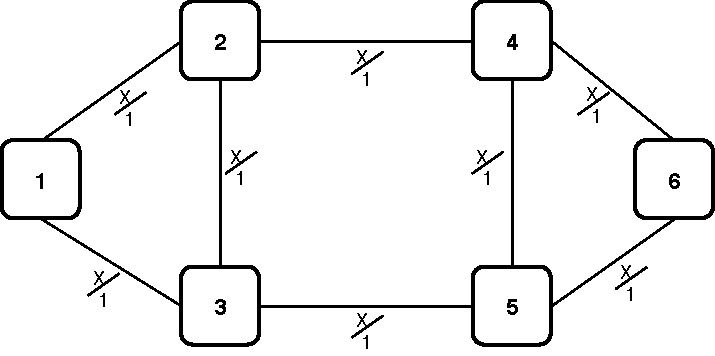
\includegraphics[width=12cm]{sdf/ilp/translucent_protection/figures/allowed_physical_topology}
\caption{Allowed physical topology. The allowed physical topology is defined by the duct and sites in the field. It is assumed that each duct supports up to 1 bidirectional transmission system and each site supports up to 1 node.}
\label{allowed3_physical_protectionmedium}
\end{figure}
\newpage
\begin{figure}[h!]
\centering
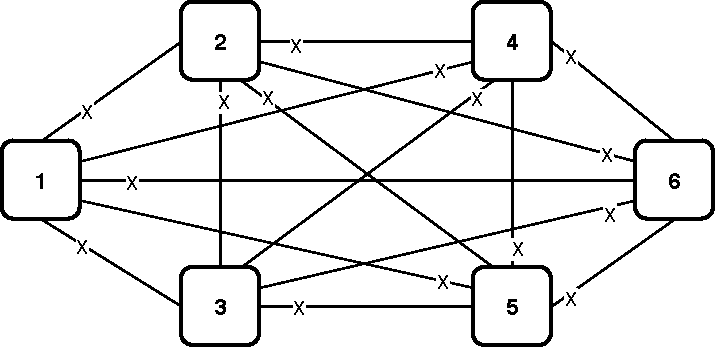
\includegraphics[width=11cm]{sdf/ilp/translucent_protection/figures/allowed_optical_topology}
\caption{Allowed optical topology. The allowed optical topology is defined by the transport mode (translucent transport mode in this case). It is assumed that each connections between demands supports up to 100 lightpaths.}
\label{allowed3_optical_protectionmedium}
\end{figure}

\begin{figure}[h!]
\centering
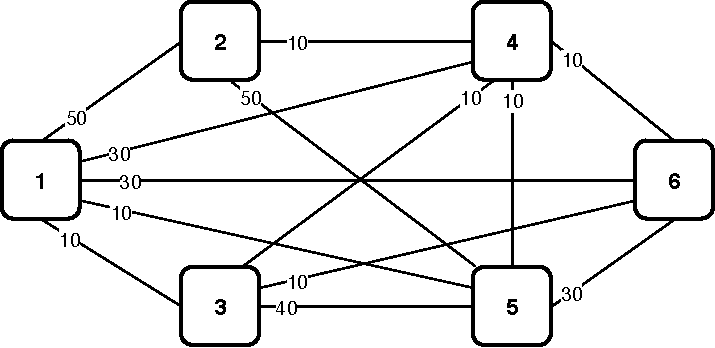
\includegraphics[width=11cm]{sdf/ilp/translucent_protection/figures/logical_topology_ODU0_medium}
\caption{ODU0 logical topology defined by the ODU0 traffic matrix.}
\label{logical3_ODU0_protectionmedium}
\end{figure}

\begin{figure}[h!]
\centering
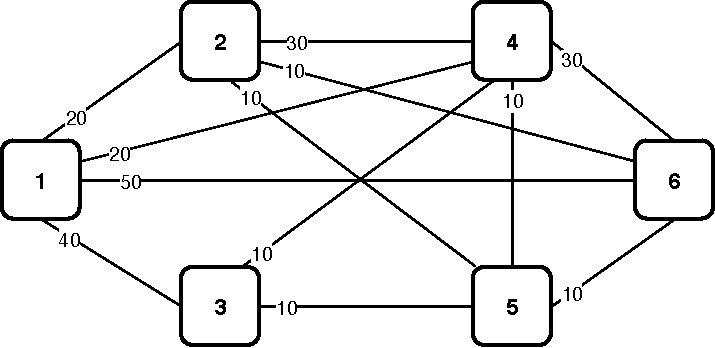
\includegraphics[width=11cm]{sdf/ilp/translucent_protection/figures/logical_topology_ODU1_medium}
\caption{ODU1 logical topology defined by the ODU1 traffic matrix.}
\label{logical3_ODU1_protectionmedium}
\end{figure}
\newpage
\begin{figure}[h!]
\centering
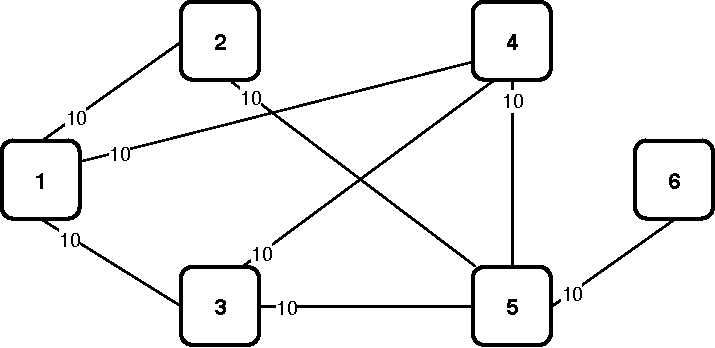
\includegraphics[width=12cm]{sdf/ilp/translucent_protection/figures/logical_topology_ODU2_medium}
\caption{ODU2 logical topology defined by the ODU2 traffic matrix.}
\label{logical3_ODU2_protectionmedium}
\end{figure}

\begin{figure}[h!]
\centering
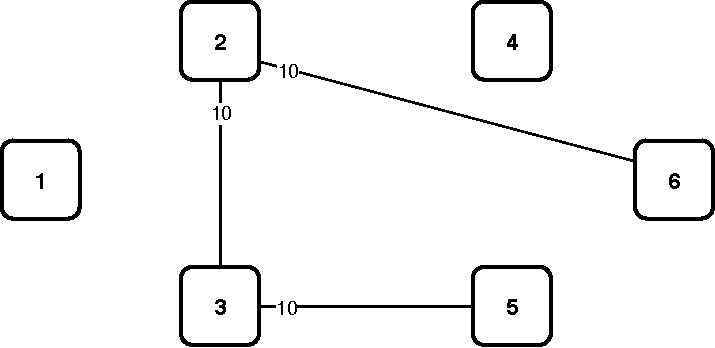
\includegraphics[width=12cm]{sdf/ilp/translucent_protection/figures/logical_topology_ODU3_medium}
\caption{ODU3 logical topology defined by the ODU3 traffic matrix.}
\label{logical3_ODU3_protectionmedium}
\end{figure}

\begin{figure}[h!]
\centering
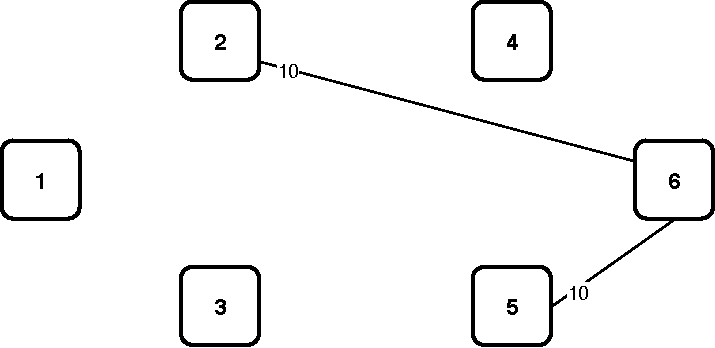
\includegraphics[width=12cm]{sdf/ilp/translucent_protection/figures/logical_topology_ODU4_medium}
\caption{ODU4 logical topology defined by the ODU4 traffic matrix.}
\label{logical3_ODU4_protectionmedium}
\end{figure}
\newpage
\begin{figure}[h!]
\centering
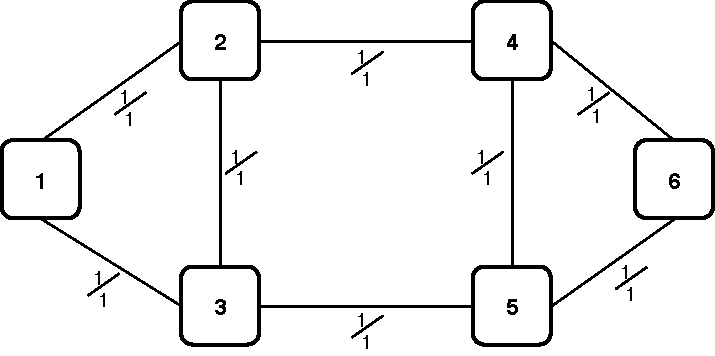
\includegraphics[width=12cm]{sdf/ilp/translucent_protection/figures/physical_topology_medium}
\caption{Physical topology after dimensioning.}
\label{physical3_protectionmedium}
\end{figure}

\begin{figure}[h!]
\centering
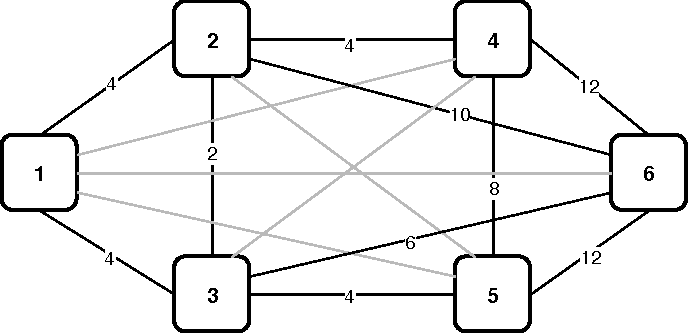
\includegraphics[width=12cm]{sdf/ilp/translucent_protection/figures/optical_topology_medium}
\caption{Optical topology after dimensioning.}
\label{optical3_protectionmedium}
\end{figure}

In table \ref{link_transluc_protec_ref_medium} we can see the number of optical channels calculated using \ref{Capex_Link} and \ref{ILPOpaque_CAPEX} and the number of amplifiers for each link calculated using \ref{Capex_amplifiers}. In the case where there are no optical channels we assume that the number of amplifiers is zero.\\

In table \ref{node_transluc_protec_ref_medium} we can see the resulting nodal degree at the physical layer, calculated based on the number of connections that the node in question performs, the number of line ports and add ports using \ref{OXC_poxc_translucp} the number of long-reach transponders using \ref{EXC_pexc2_translucp} and the number of tributary ports using \ref{EXC_pexc1_translucp}.\\
\newpage
\begin{table}[h!]
\centering
\begin{tabular}{|| c | c | c ||}
 \hline
 \multicolumn{3}{|| c ||}{Information regarding links} \\
 \hline
 \hline
 Bidirectional Link & Optical Channels & Amplifiers\\
 \hline
 Node 1 <-> Node 2 & 4 & 4 \\
 Node 1 <-> Node 3 & 4 & 6 \\
 Node 2 <-> Node 3 & 2 & 0 \\
 Node 2 <-> Node 4 & 14 & 6 \\
 Node 3 <-> Node 5 & 10 & 8 \\
 Node 4 <-> Node 5 & 8 & 1 \\
 Node 4 <-> Node 6 & 22 & 7 \\
 Node 5 <-> Node 6 & 18 & 3 \\
 \hline
\end{tabular}
\caption{Table with information regarding links for translucent mode with 1+1 protection.}
\label{link_transluc_protec_ref_medium}
\end{table}

\begin{table}[h!]
\centering
\begin{tabular}{|| c | c | c | c | c | c ||}
 \hline
 \multicolumn{6}{|| c ||}{Information regarding nodes} \\
 \hline
 \hline
 \multicolumn{2}{|| c |}{ } & \multicolumn{2}{ c |}{Electrical part} & \multicolumn{2}{ c ||}{Optical part} \\
 \hline
 Node & Resulting Nodal Degree & Tributary Ports & LR Transponders & Add Ports & Line Ports\\
 \hline
 1 & 2 & 290 & 8 & 8 & 8 \\
 2 & 3 & 230 & 20 & 20 & 20 \\
 3 & 3 & 180 & 16 & 16 & 16 \\
 4 & 3 & 200 & 24 & 24 & 44 \\
 5 & 3 & 240 & 24 & 24 & 36 \\
 6 & 2 & 220 & 40 & 40 & 40 \\
\hline
\end{tabular}
\caption{Table with information regarding nodes for translucent mode with 1+1 protection.}
\label{node_transluc_protec_ref_medium}
\end{table}

Through the information obtained previously on the nodes we can now create tables with detailed information about each node. In each table mentioned below we can see how many ports are connected to a given node and its bit rate (in relation to the line ports) and how many ports are assigned to each different bit rate (in relation to the tributary ports).\\

\newpage
\begin{table}[h!]
\centering
\begin{tabular}{|| c | c | c ||}
 \hline
 \multicolumn{3}{|| c ||}{Detailed description of Node 1} \\
 \hline
 \hline
 Electrical part & Number of total demands & Bit rate \\
 \hline
\multirow{3}{*}{290 tributary ports} & 130 & ODU0 \\
 & 130 & ODU1 \\
 & 30 & ODU2 \\
 \hline
  & Node<--Optical Channels-->Node & Bit rate \\
 \hline
\multirow{2}{*}{8 LR Transponders} & 1  <---- 4 ---->  2 & \multirow{2}{*}{100 Gbits/s} \\
  & 1  <---- 4 ---->  3 & \\
 \hline
 \hline
 Optical part & Node<--Optical Channels-->Node & Bit rate \\
 \hline
 \multirow{2}{*}{8 add ports} & 1  <---- 4 ---->  2 & \multirow{4}{*}{100 Gbits/s} \\
  & 1  <---- 4 ---->  3 & \\ \cline{1-2}
 \multirow{2}{*}{8 line ports} & 1  <---- 4 ---->  2 & \\
  & 1  <---- 4 ---->  3 & \\
\hline
\end{tabular}
\caption{Table with detailed description of node 1. The number of demands is distributed to the various destination nodes, this distribution can be observed in section \ref{medium_traffic_scenario}.}
\end{table}
\newpage
\begin{table}[h!]
\centering
\begin{tabular}{|| c | c | c ||}
 \hline
 \multicolumn{3}{|| c ||}{Detailed description of Node 2} \\
 \hline
 \hline
 Electrical part & Number of total demands & Bit rate \\ \hline
\multirow{5}{*}{230 tributary ports} & 110 & ODU0 \\
 & 70 & ODU1 \\
 & 20 & ODU2 \\
 & 20 & ODU3 \\
 & 10 & ODU4 \\
 \hline
  & Node<--Optical Channels-->Node & Bit rate \\
  \hline
\multirow{4}{*}{20 LR Transponders} & 2  <---- 4 ---->  1 & \multirow{4}{*}{100 Gbits/s} \\
  & 2  <---- 2 ---->  3 & \\
  & 2  <---- 4 ---->  4 & \\
  & 2  <---- 10 ---->  6 & \\
 \hline
 \hline
 Optical part & Node<--Optical Channels-->Node & Bit rate \\
 \hline
 \multirow{4}{*}{20 add ports} & 2  <---- 4 ---->  1 & \multirow{8}{*}{100 Gbits/s} \\
  & 2  <---- 2 ---->  3 & \\
  & 2  <---- 4 ---->  4 & \\
  & 2  <---- 10 ---->  6 & \\ \cline{1-2}
 \multirow{4}{*}{20 line ports} & 2  <---- 4 ---->  1 & \\
  & 2  <---- 2 ---->  3 & \\
  & 2  <---- 4 ---->  4 & \\
  & 2  <---- 10 ---->  6 & \\
\hline
\end{tabular}
\caption{Table with detailed description of node 2. The number of demands is distributed to the various destination nodes, this distribution can be observed in section \ref{medium_traffic_scenario}.}
\end{table}
\newpage
\begin{table}[h!]
\centering
\begin{tabular}{|| c | c | c ||}
 \hline
 \multicolumn{3}{|| c ||}{Detailed description of Node 3} \\
 \hline
 \hline
 Electrical part & Number of total demands & Bit rate \\
 \hline
 \multirow{4}{*}{180 tributary ports} & 70 & ODU0 \\
 & 60 & ODU1\\
 & 30 & ODU2\\
 & 20 & ODU3\\
 \hline
  & Node<--Optical Channels-->Node & Bit rate \\ \hline
 \multirow{4}{*}{16 LR Transponders} & 3  <---- 4 ---->  1 & \multirow{4}{*}{100 Gbits/s} \\
  & 3  <---- 2 ---->  2 & \\
  & 3  <---- 4 ---->  5 & \\
  & 3  <---- 6 ---->  6 & \\
 \hline
 \hline
 Optical part & Node<--Optical Channels-->Node & Bit rate \\
 \hline
 \multirow{4}{*}{16 add ports} & 3  <---- 4 ---->  1 & \multirow{8}{*}{100 Gbits/s} \\
  & 3  <---- 2 ---->  2 & \\
  & 3  <---- 4 ---->  5 & \\
  & 3  <---- 6 ---->  6 & \\ \cline{1-2}
 \multirow{4}{*}{16 line ports} & 3  <---- 4 ---->  1 & \\
  & 3  <---- 2 ---->  2 & \\
  & 3  <---- 4 ---->  5 & \\
  & 3  <---- 6 ---->  6 & \\
\hline
\end{tabular}
\caption{Table with detailed description of node 3. The number of demands is distributed to the various destination nodes, this distribution can be observed in section \ref{medium_traffic_scenario}.}
\end{table}

\newpage
\begin{table}[h!]
\centering
\begin{tabular}{|| c | c | c ||}
 \hline
 \multicolumn{3}{|| c ||}{Detailed description of Node 4} \\
 \hline
 \hline
 Electrical part & Number of total demands & Bit rate \\ \hline
\multirow{3}{*}{200 tributary ports} & 70 & ODU0 \\
 & 100 & ODU1 \\
 & 30 & ODU2 \\
 \hline
  & Node<--Optical Channels-->Node & Bit rate \\ \hline
 \multirow{3}{*}{24 LR Transponders} & 4  <---- 4 ---->  2 & \multirow{3}{*}{100 Gbits/s} \\
  & 4  <---- 8 ---->  5 & \\
  & 4  <---- 12 ---->  6 & \\
 \hline
 \hline
 Optical part & Node<--Optical Channels-->Node & Bit rate \\
 \hline
 \multirow{3}{*}{24 add ports} & 4  <---- 4 ---->  2 & \multirow{7}{*}{100 Gbits/s} \\
  & 4  <---- 8 ---->  5 & \\
  & 4  <---- 12 ---->  6 & \\ \cline{1-2}
 \multirow{4}{*}{44 line ports} & 4  <---- 4 ---->  2 & \\
  & 4  <---- 8 ---->  5 & \\
  & 4  <---- 12 ---->  6 & \\
  & 2  <---- 10 ---->  6 & \\
\hline
\end{tabular}
\caption{Table with detailed description of node 4. The number of demands is distributed to the various destination nodes, this distribution can be observed in section \ref{medium_traffic_scenario}.}
\end{table}

\newpage
\begin{table}[h!]
\centering
\begin{tabular}{|| c | c | c ||}
 \hline
 \multicolumn{3}{|| c ||}{Detailed description of Node 5} \\
 \hline
 \hline
 Electrical part & Number of total demands & Bit rate \\ \hline
\multirow{5}{*}{240 tributary ports} & 140 & ODU0 \\
 & 40 & ODU1 \\
 & 40 & ODU2 \\
 & 10 & ODU3 \\
 & 10 & ODU4 \\
 \hline
  & Node<--Optical Channels-->Node & Bit rate \\ \hline
 \multirow{3}{*}{24 LR Transponders} & 5  <---- 4 ---->  3 & \multirow{3}{*}{100 Gbits/s} \\
  & 5  <---- 8 ---->  4 & \\
  & 5  <---- 12 ---->  6 & \\
 \hline
 \hline
 Optical part & Node<--Optical Channels-->Node & Bit rate \\
 \hline
 \multirow{3}{*}{24 add ports} & 5  <---- 4 ---->  3 & \multirow{7}{*}{100 Gbits/s} \\
  & 5  <---- 8 ---->  4 & \\
  & 5  <---- 12 ---->  6 & \\ \cline{1-2}
 \multirow{4}{*}{36 line ports} & 5  <---- 4 ---->  3 & \\
  & 5  <---- 8 ---->  4 & \\
  & 5  <---- 12 ---->  6 & \\
  & 3  <---- 6 ---->  6 & \\
\hline
\end{tabular}
\caption{Table with detailed description of node 5. The number of demands is distributed to the various destination nodes, this distribution can be observed in section \ref{medium_traffic_scenario}.}
\end{table}

\newpage
\begin{table}[h!]
\centering
\begin{tabular}{|| c | c | c ||}
 \hline
 \multicolumn{3}{|| c ||}{Detailed description of Node 6} \\
 \hline
 \hline
 Electrical part & Number of total demands & Bit rate \\ \hline
\multirow{5}{*}{220 tributary ports} & 80 & ODU0 \\
 & 100 & ODU1 \\
 & 10 & ODU2 \\
 & 10 & ODU3 \\
 & 20 & ODU4 \\
 \hline
  & Node<--Optical Channels-->Node & Bit rate \\ \hline
 \multirow{3}{*}{20 LR Transponders} & 6  <---- 4 ---->  2 & \multirow{3}{*}{100 Gbits/s} \\
  & 6  <---- 2 ---->  4 & \\
  & 6  <---- 14 ---->  5 & \\
 \hline
 Optical part & Node<--Optical Channels-->Node & Bit rate \\
 \hline
 \multirow{3}{*}{20 add ports} & 6  <---- 4 ---->  2 & \multirow{6}{*}{100 Gbits/s} \\
  & 6  <---- 2 ---->  4 & \\
  & 6  <---- 14 ---->  5 & \\ \cline{1-2}
 \multirow{3}{*}{20 line ports} & 6  <---- 4 ---->  2 & \\
  & 6  <---- 2 ---->  4 & \\
  & 6  <---- 14 ---->  5 & \\
\hline
\end{tabular}
\caption{Table with detailed description of node 6. The number of demands is distributed to the various destination nodes, can be observed in section \ref{medium_traffic_scenario}.}
\end{table}

Finally through table \ref{scripttransluc_protec_ref_medium} we can see the CAPEX result for this model.
\begin{table}[h!]
\centering
\begin{tabular}{|| c | c | c | c | c | c | c ||}
 \hline
 \multicolumn{7}{|| c ||}{CAPEX of the Network} \\
 \hline
 \hline
 \multicolumn{3}{|| c |}{ } & Quantity & Unit Price & Cost & Total \\
 \hline
 \multirow{3}{*}{Link Cost} & \multicolumn{2}{ c |}{OLTs} & 16 & 15 000 \euro & 240 000 \euro & \multirow{3}{*}{82 520 000 \euro} \\ \cline{2-6}
 & \multicolumn{2}{ c |}{100 Gbits/s Transceivers} & 164 & 5 000 \euro/Gbit/s & 82 000 000 \euro & \\ \cline{2-6}
 & \multicolumn{2}{ c |}{Amplifiers} & 70 & 4 000 \euro & 280 000 \euro & \\
 \hline
 \multirow{10}{*}{Node Cost} & \multirow{7}{*}{Electrical} & EXCs & 6 & 10 000 \euro & 60 000 \euro & \multirow{10}{*}{14 145 900 \euro} \\ \cline{3-6}
 & & ODU0 Ports & 600 & 10 \euro/port & 6 000 \euro & \\ \cline{3-6}
 & & ODU1 Ports & 500 & 15 \euro/port & 7 500 \euro & \\ \cline{3-6}
 & & ODU2 Ports & 160 & 30 \euro/port & 4 800 \euro & \\ \cline{3-6}
 & & ODU3 Ports & 60 & 60 \euro/port & 3 600 \euro & \\ \cline{3-6}
 & & ODU4 Ports & 40 & 100 \euro/port & 4 000 \euro & \\ \cline{3-6}
 & &Transponders& 132 & 100 000 \euro/port & 13 200 000 \euro & \\ \cline{2-6}
 & \multirow{3}{*}{Optical} & OXCs & 6 & 20 000 \euro & 120 000 \euro & \\ \cline{3-6}
 & & Line Ports & 164 & 2 500 \euro/port & 410 000 \euro & \\ \cline{3-6}
 & & Add Ports & 132 & 2 500 \euro/port & 330 000 \euro & \\
 \hline
 \multicolumn{6}{|| c |}{Total Network Cost} & 96 665 900 \euro \\
\hline
\end{tabular}
\caption{Table with detailed description of CAPEX for this scenario.}
\label{scripttransluc_protec_ref_medium}
\end{table}
\newpage
\begin{table}[h]
\centering
\begin{tabular}{||c|c|c|c|c||}
 \hline
 \multicolumn{5}{|| c ||}{Routing} \\
 \hline
 \hline
 o & d & Type & Links & Demands \\
 \hline
 \multirow{2}{*}{1}&\multirow{2}{*}{2}&W&\{(1,3),(3,5),(5,6),(6,4),(4,2)\}&50 ODU0, 20 ODU1, 10 ODU2\\
  & &P& \{(1,2)\} &50 ODU0, 20 ODU1, 10 ODU2 \\ \hline
 \multirow{2}{*}{1}&\multirow{2}{*}{3}&W& \{(1,2),(2,3)\} & 10 ODU0, 40 ODU1, 10 ODU2\\
  & &P& \{(1,3)\} & 10 ODU0, 40 ODU1, 10 ODU2 \\ \hline
 \multirow{2}{*}{1} & \multirow{2}{*}{4}&W&\{(1,3),(3,5),(5,6),(6,4)\}&30 ODU0, 20 ODU1, 10 ODU2\\
  & &P& \{(1,2),(2,4)\} & 30 ODU0, 20 ODU1, 10 ODU2 \\ \hline
 \multirow{2}{*}{1} & \multirow{2}{*}{5}&W&\{(1,2),(2,4),(4,5)\}& 10 ODU0\\
  & &P& \{(1,3),(3,5)\} & 10 ODU0 \\ \hline
 \multirow{2}{*}{1} & \multirow{2}{*}{6}&W& \{(1,3),(3,5),(5,6)\} & 30 ODU0, 50 ODU1 \\
  & &P& \{(1,2),(2,4),(4,6)\} & 30 ODU0, 50 ODU1 \\ \hline
 \multirow{4}{*}{2} & \multirow{4}{*}{3}&W& \{(2,1),(1,3)\} & 5 ODU3 \\
  & &W& \{(2,4),(4,6),(6,5),(5,3)\} & 5 ODU3 \\
  & &P& \{(2,3)\} & 5 ODU3 \\
  & &P& \{(2,1),(1,3)\} & 5 ODU3 \\ \hline
 \multirow{2}{*}{2} & \multirow{2}{*}{4}&W&\{(2,4),(4,6),(6,4)\}&10 ODU0, 30 ODU1 \\
  & &P& \{(2,4)\} & 10 ODU0, 30 ODU1 \\ \hline
 \multirow{4}{*}{2} & \multirow{4}{*}{5}&W&\{(2,4),(4,5)\} & 50 ODU0, 10 ODU1 \\
  & &W& \{(2,1),(1,3),(3,5)\} & 1 ODU2 \\
  & &P& \{(2,3),(3,5)\} & 50 ODU0, 10 ODU1 \\
  & &P& \{(2,4),(4,5)\} & 1 ODU2 \\ \hline
 \multirow{4}{*}{2} & \multirow{4}{*}{6}&W&\{(2,3),(3,5),(5,6)\}& 10 ODU1, 2 ODU4 \\
  & &W& \{(2,4),(4,6)\} & 10 0DU3, 4 ODU4 \\
  & &W& \{(2,1),(1,3),(3,5),(5,6)\} & 4 ODU4 \\
  & &P& \{(2,4),(4,6)\} & 10 ODU1, 10 ODU3, 10 ODU4 \\ \hline
 \multirow{2}{*}{3} & \multirow{2}{*}{4}&W& \{(3,5),(5,6),(6,4)\} & 10 ODU0, 10 ODU1, 10 ODU2 \\
  & &P& \{(3,2),(2,4)\} & 10 ODU0, 10 ODU1, 10 ODU2 \\ \hline
 \multirow{3}{*}{3}&\multirow{3}{*}{5}&W&\{(3,2),(2,4),(4,5)\}&40 ODU0, 10 ODU1 \\
  & &W& \{(3,5),(5,6),(6,4),(4,5)\}& 10 ODU2, 10 ODU3\\
  & &P& \{(3,5)\} & 40 ODU0, 10 ODU1, 10 ODU2, 10 ODU3 \\ \hline
 \multirow{2}{*}{3} & \multirow{2}{*}{6}&W& \{(3,2),(2,4),(4,6)\} & 10 ODU0 \\
  & &P& \{(3,6)\} & 10 ODU0 \\ \hline
 \multirow{3}{*}{4} & \multirow{3}{*}{5}&W& \{(4,2),(2,3),(3,5)\} & 10 ODU0 \\
  & &W& \{(4,6),(6,5),(5,3),(3,5)\} & 10 ODU1, 10 ODU2 \\
  & &P& \{(4,5)\} & 10 ODU0, 10 ODU1, 10 ODU2 \\ \hline
 \multirow{2}{*}{4} & \multirow{2}{*}{6}&W& \{(4,2),(2,4),(4,6)\} & 10 ODU0, 30 ODU1\\
  & &P& \{(4,6)\} & 10 ODU0, 30 ODU1\\ \hline
 \multirow{3}{*}{5} & \multirow{3}{*}{6}&W&\{(5,3),(3,5),(5,6)\}& 30 ODU0, 10 ODU1, 10 ODU2, 2 ODU4 \\
  & &W& \{(5,4),(4,6)\} & 8 ODU4 \\
  & &P& \{(5,6)\}& 30 ODU0, 10 ODU1, 10 ODU2, 10 ODU4 \\ \hline
\end{tabular}
\caption{Table with description of demands routing. The type W means that it is working path and type P protection path.}
\label{path_transluc_protec_ref_medium}
\end{table}

\newpage
\newpage
\newpage
\newpage
\textbf{High Traffic Scenario:}\\

In this scenario we have to take into account the traffic calculated in \ref{high_traffic_scenario}. In a first phase we will show the various existing topologies of the network. The first are the allowed topologies, physical and optical topology, the second are the logical topology for all ODUs and finally the resulting physical and optical topology.

\begin{figure}[h!]
\centering
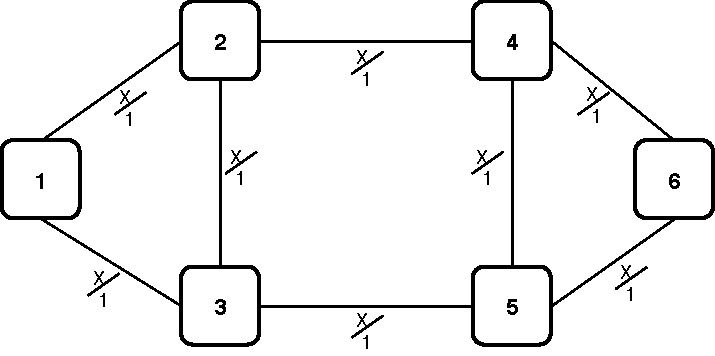
\includegraphics[width=12cm]{sdf/ilp/translucent_protection/figures/allowed_physical_topology}
\caption{Allowed physical topology. The allowed physical topology is defined by the duct and sites in the field. It is assumed that each duct supports up to 1 bidirectional transmission system and each site supports up to 1 node.}
\label{allowed3_physical_protectionhigh}
\end{figure}
\newpage
\begin{figure}[h!]
\centering
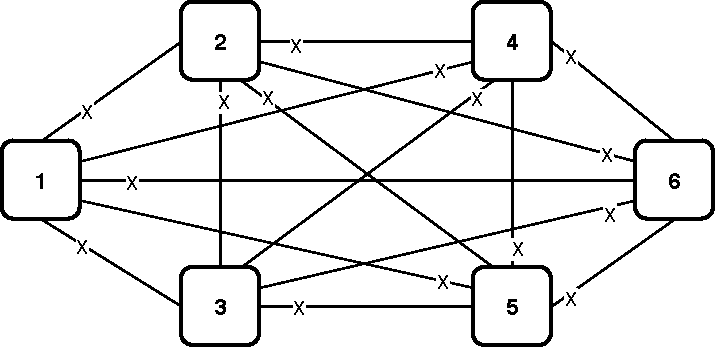
\includegraphics[width=11cm]{sdf/ilp/translucent_protection/figures/allowed_optical_topology}
\caption{Allowed optical topology. The allowed optical topology is defined by the transport mode (translucent transport mode in this case). It is assumed that each connections between demands supports up to 100 lightpaths.}
\label{allowed3_optical_protectionhigh}
\end{figure}

\begin{figure}[h!]
\centering
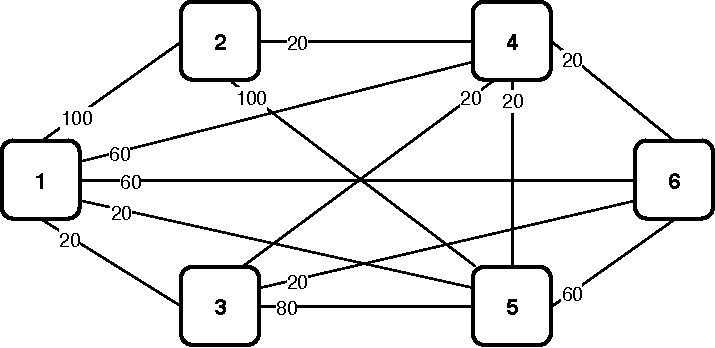
\includegraphics[width=11cm]{sdf/ilp/translucent_protection/figures/logical_topology_ODU0_high}
\caption{ODU0 logical topology defined by the ODU0 traffic matrix.}
\label{logical3_ODU0_protectionhigh}
\end{figure}

\begin{figure}[h!]
\centering
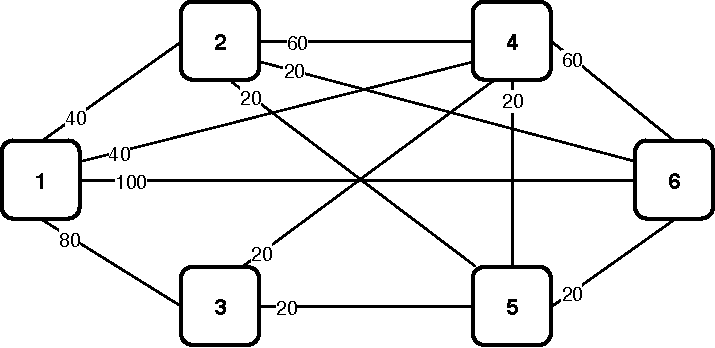
\includegraphics[width=11cm]{sdf/ilp/translucent_protection/figures/logical_topology_ODU1_high}
\caption{ODU1 logical topology defined by the ODU1 traffic matrix.}
\label{logical3_ODU1_protectionhigh}
\end{figure}
\newpage
\begin{figure}[h!]
\centering
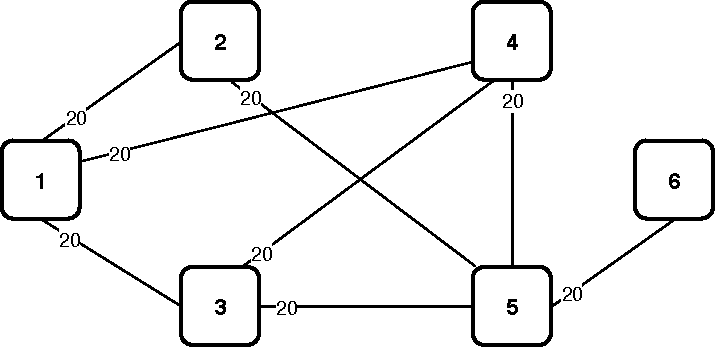
\includegraphics[width=12cm]{sdf/ilp/translucent_protection/figures/logical_topology_ODU2_high}
\caption{ODU2 logical topology defined by the ODU2 traffic matrix.}
\label{logical3_ODU2_protectionhigh}
\end{figure}

\begin{figure}[h!]
\centering
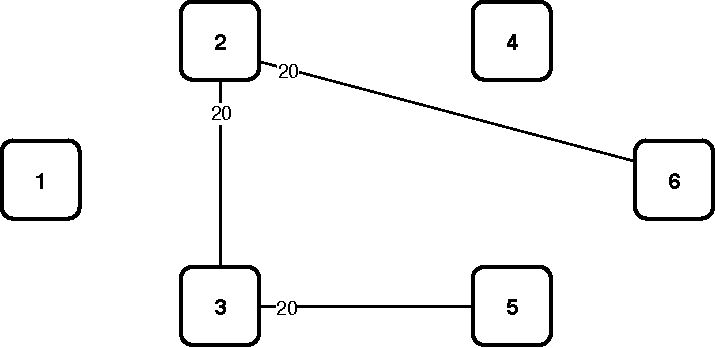
\includegraphics[width=12cm]{sdf/ilp/translucent_protection/figures/logical_topology_ODU3_high}
\caption{ODU3 logical topology defined by the ODU3 traffic matrix.}
\label{logical3_ODU3_protectionhigh}
\end{figure}

\begin{figure}[h!]
\centering
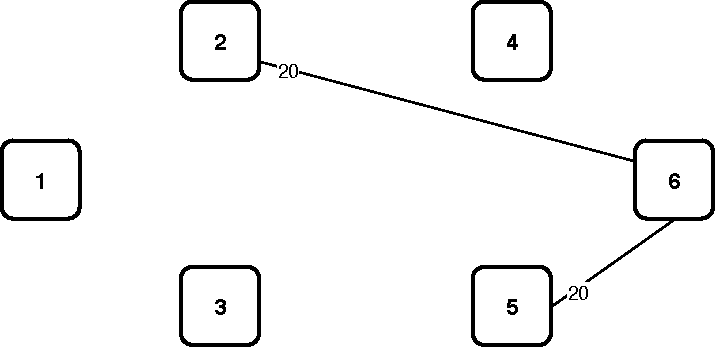
\includegraphics[width=12cm]{sdf/ilp/translucent_protection/figures/logical_topology_ODU4_high}
\caption{ODU4 logical topology defined by the ODU4 traffic matrix.}
\label{logical3_ODU4_protectionhigh}
\end{figure}
